\section{Theorie}
\label{sec:Theorie}

In diesem Versuch wird das Relaxationsverhalten eines RC-Kreises untersucht.
Relaxation beschreibt allgemein die nicht-oszillatorische Rückkehr eines Systems in seinen Ausgangszustand.
Die Änderung der betrachteten Größe ist meistens proportional zur Zeit $t$, somit ergibt sich eine asymptotische
Annährung an den Ausgangszustand.\cite{v353}

\subsection{Auf- und Entladen eines Kondensators}
Ein wichtiges Beispiel für Relaxationsvorgänge ist das Entladen eines zuvor aufgeladenen Kondensators im RC- Kreis.
Ein RC Kreis besteht aus einem Widerstand $R$ und einem Kondensator mit der Kapazität $C$ sowie einem Schalter, um zwischen 
Auf- und Entladen zu wechseln:
\begin{figure}
    \centering
    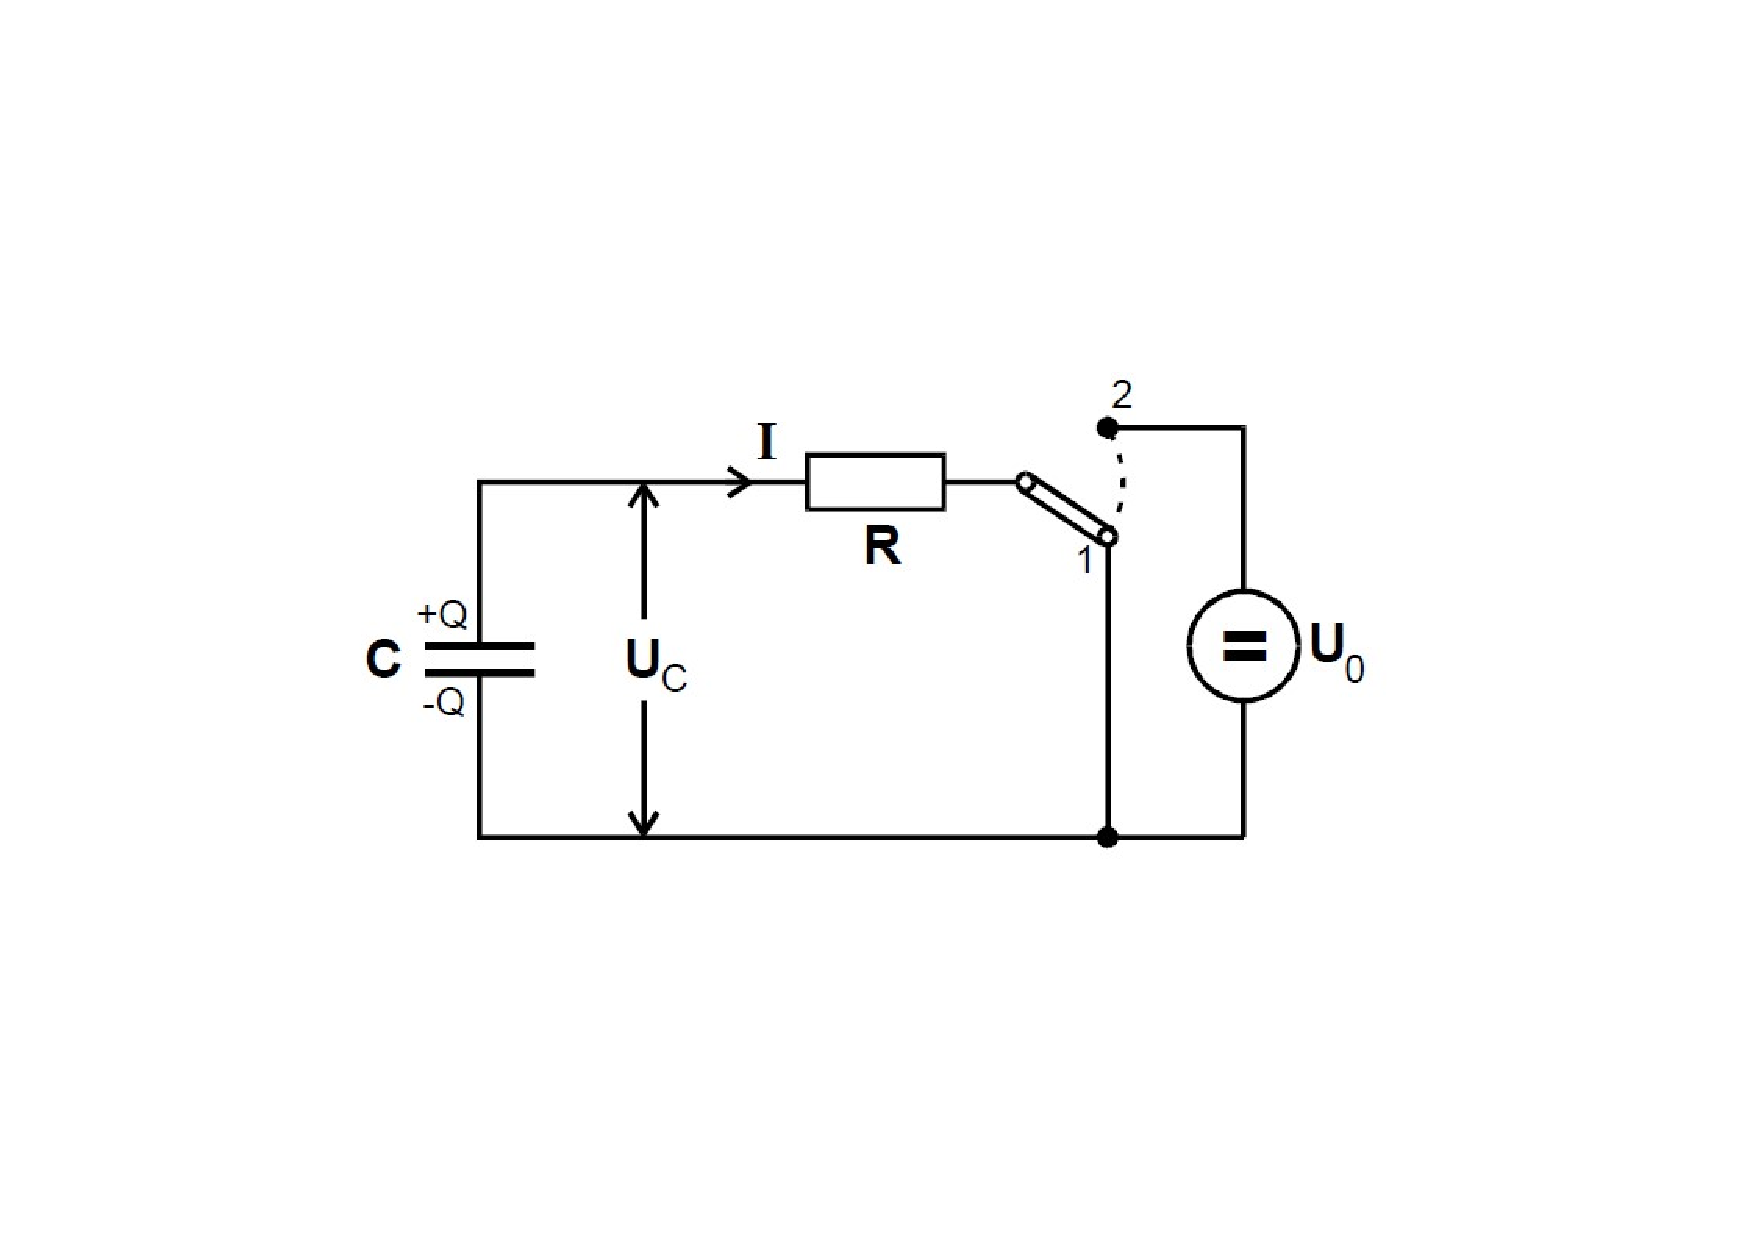
\includegraphics[height=8cm]{content/Theorie - RC-Kreis.pdf}
    \caption{RC Kreis mit Schalter \cite{v353}}
    \label{fig:Theorie - RC_Kreis}
\end{figure}

Der Spannungsverlauf beim Entladen ist gegeben durch:

\begin{equation}
    U(t)= U_{0}e^{-\frac{1}{RC}t} . \label{eqn:Entladen}
\end{equation}

Beim Aufladen lautet die Formel:

\begin{equation}
    U(t)= U_{0}(1-e^{-\frac{1}{RC}t}) . \label{eqn:Aufladen}
\end{equation}

Dabei beschreibt $RC$ die Zeitkonstante $c$, diese ist das Maß für die Geschwindigkeit mit der das System seinem
Ausgangszustand zustrebt und soll in diesem Versuch experimentell ermittelt werden.
Außerdem wird das öffnen/schließen des Schalters durch das anlegen einer Rechtecksspannung ersetzt.

\subsection{Relaxationsvorgänge bei periodischer Auslenkung}
Nun wird der RC-Kreis mit Wechselspannung $U(t) = U_{0}\cos(\omega t)$ betrieben:
\begin{figure}
    \centering
    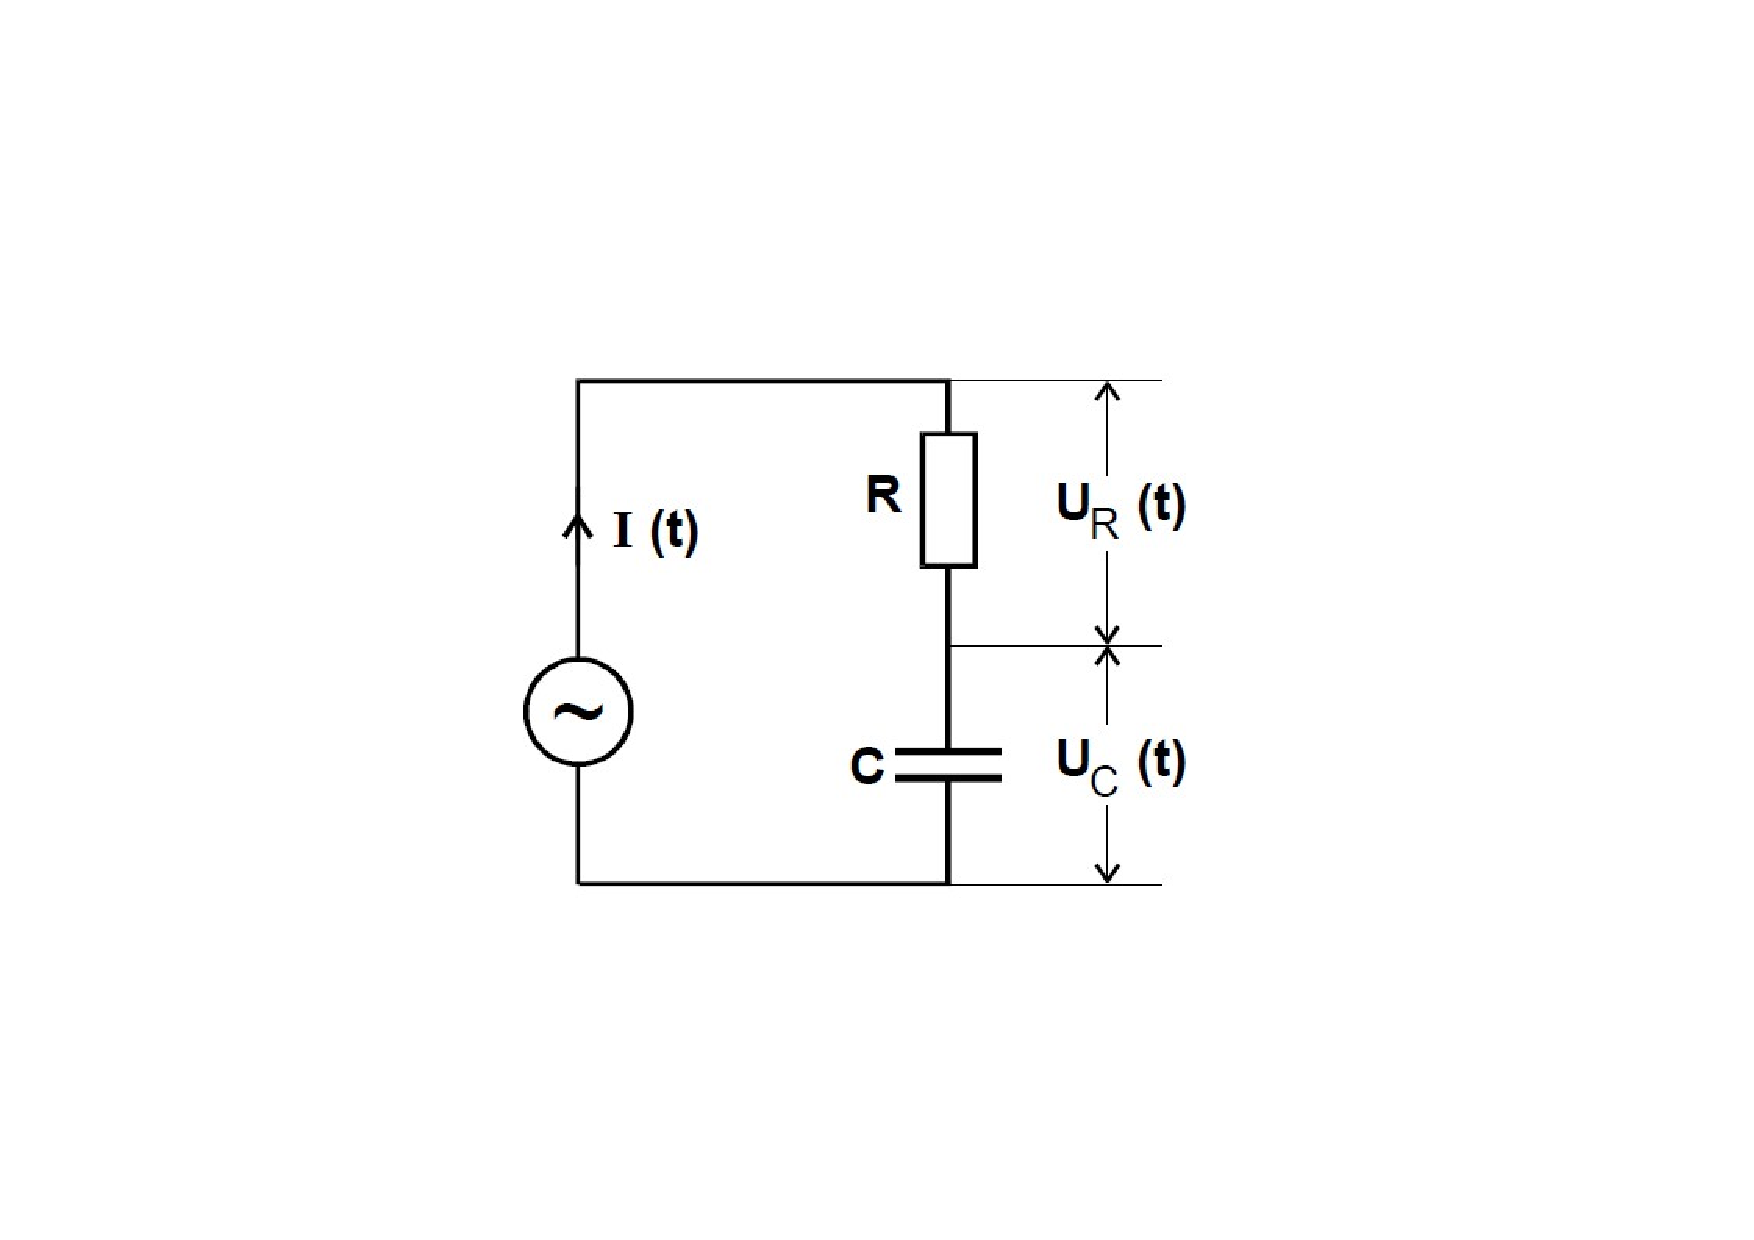
\includegraphics{content/Theorie - RC-Kreis Wechselspannung.pdf}
    \caption{RC Kreis mit angelegter Wechselspannung \cite{v353}}
    \label{fig:Theorie - RC_Kreis Wechselspannung}
\end{figure}

Die Amplitude $A$ der am Kondensator gemessenen Spannung $U_{C}(t)$ hängt von der Frequenz $\omega$ der Wechselspannung ab:

\begin{equation}
    A(\omega)= \frac{U_{0}}{\sqrt{1+\omega ^{2}R^{2}C^{2}}} . \label{eqn:Tiefpass}
\end{equation}

Zusätzlich ergibt sich ein Phasenversatz $\varphi$ der Kondensatorspannung $U_{C}(t)$ und der angelegten Spannung $U(t)$
in Abhängigkeit von der Frequenz $\omega$:

\begin{equation}
    \varphi (\omega )=\arctan (-\omega RC). \label{eqn:Phasenversatz}
\end{equation}

Für kleine Frequenzen bleibt die Amplitude $A$ also unverändert, bei wachsender Frequenz $\omega$ nimmt sie ab während
der Phasenversatz $\varphi$ größer wird. Für sehr große $\omega$ geht $A$ gegen Null und der Phasenversatz beträgt $\frac{\pi}{2}$.
Dieser Verlauf wird in der Auswertung graphisch dargestellt und ebenfalls verwendet, um die Zeitkonstante $RC$ zu bestimmen.

Aufgrund des beschriebenen Verhaltens wird ein solcher RC-Kreis mit Wechselspannung auch als Tiefpass bezeichnet, weil die angelegte
Spannung für niedrige Frequenzen ohne Phasenversatz durchgelassen wird.

\subsection{Der RC Kreis als Integrationsglied}
\label{sec:theorie-integration}
Für Frequenzen $\omega >> 1/RC$ kann man näherungsweise schreiben:

\begin{equation}
    U_{C}(t) = \frac{1}{RC}\int_{0}^{t}U({t}')d{t}'. \label{eqn:Integrator}
\end{equation}

Der RC-Kreis ist also in der Lage, die angelegte Spannung $U(t)$ zu integrieren. Dies folgt direkt aus \ref{eqn:Integrator},
da die Kondensatorspannung $U_{C}(t)$ proportional zum Integral der angelegten Spannug, also $\int U(t)dt$, ist.
Dieses Verhalten wird im Versuch graphisch untersucht.